\chapter{Problem formalization}\label{ch:problem-formalization}

The problem with implementation of optimization algorithms in applications is that their
performance requirements are quite high and are fully utilized only while working.
Optimization algorithm is not running all the time and for that reason hardware resources are mainly unused.
These unused resources could be potentially used by another instance of algorithm
or can be shutdown completely to reduce hosting costs.
Also adding more time to the job execution does not always bring better solution
but it certainly costs more.

The figure \ref{fig:problem-scheme} displays standard case,
when application is deployed on the server.
Because the application uses optimization algorithm, 
the server must be powerful enough to deliver suitable results.
This also means,
that the server resources must be allocated to the application and to nothing else,
which leads to the resource wasting.
\begin{figure}[ht] 
    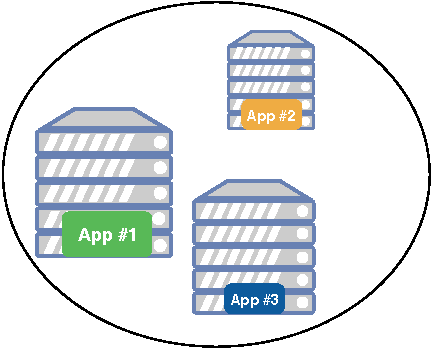
\includegraphics[scale=0.7]{i_problem_scheme_without.pdf} 
    \centering
    \caption{Problem visualization}
    \label{fig:problem-scheme}
\end{figure}

The next figure \ref{fig:problem-with-load-balancer} visualizes scenario when the load balancer is used.
Instead of using powerful servers for each of the applications,
it is enough to use small server or even deploy multiple applications on the one machine.
This can be done thanks to the outsourcing of the optimization jobs to the external servers with more computational power.
\begin{figure}[ht] 
    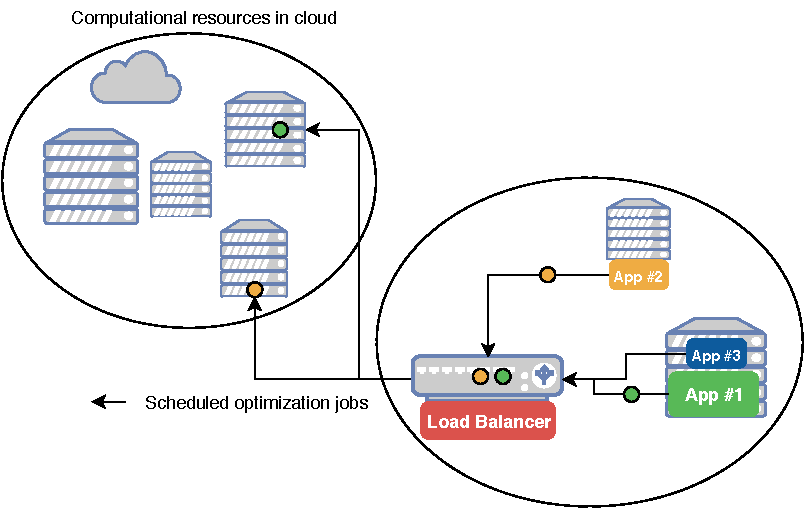
\includegraphics[width=\textwidth]{i_problem_scheme_jobs.pdf} 
    \centering
    \caption{Problem visualization with the load balancer}
    \label{fig:problem-with-load-balancer}
\end{figure}
The circles are optimization jobs,
that were triggered by the same colored applications
and are being executed on the different servers in the cloud.

Moreover,
as can be seen in the figure \ref{fig:problem-with-load-balancer},
these servers do not need to be allocated all the time.
Most resources providers, 
such as AWS\cite{awsReference} or Azure\cite{azureReference} allow to reallocate hardware on the fly.
This leads to potentially significant cost savings 
and ultimately to the more effective infrastructure.

%%
%% Author: lukas
%% 12.02.2019
%%

\section{Formal definition}\label{sec:formal-definition}
\begin{itemize}
    \item $T_{\max}$ - maximal optimization job execution time provided by user and specified before execution started

    \item $T$ - actual optimization job execution time, when no execution time optimization is being used $T = T_{\max}$

    \item $RC$ - \textit{Resource Costs} - all hardware costs used for executing optimization job by some algorithm
    \todo{don't know how to say that - costs that you actually pay for hardware}
    \begin{equation}
        RC = \sum_{i=0}^T RC_i
    \end{equation}

    \item $RC_t$ - \textit{Resource Costs} in time $t$ - accumulated costs from beginning of execution to time $t$
    \begin{equation}
        RC_{t} = \sum_{i=0}^{t-1} RC_i
    \end{equation}

    \item $RC_{\max}$ - maximal resource costs specified by user in advance
    \begin{equation}
        RC_{\max} \geq RC
    \end{equation}

    \item $V$ - \textit{Solution Value} - value of the found solution, since this paper focus on cost optimization,
    \textit{Solution Value} is cost of found solution
    \begin{equation}
        V = min \{ V_t \}, \quad t = 0 \dots T
    \end{equation}

    \item $V_t$ - \textit{Solution Value} in time $t$ - best solution provided by algorithm since the beginning of the job execution
    until time $t$

\end{itemize}

Then load balancer optimizes following function

\begin{equation}
    min \{ \alpha RC + \beta V \,|\, \alpha, \beta \in \mathbb{R} \}
\end{equation}

Where $\alpha$ and $\beta$ are coefficients that are balancing $RC$ and $V$.



%TODO define load balancer requirements
%\subsection{Load Balancer Requirements}\label{subsec:load-balancer-requirements}
% For successful server implementation we must enforce following things
% \begin{itemize}
%    \item Running optimization algorithms can't interfere with each other
%    \item RMS guarantee that scheduled job will be always executed
%    \item
% \end{itemize}


\section{Resulting problem}\label{sec:resulting-problem}
Proposed formal definition (\ref{sec:formal-definition}) implies that problem is 
integer linear problem with job execution cost as its main optimization criteria. 
These problems are solvable by various types of mixed integer linear programming solvers.
Linear optimization and its characteristics are outlined in previous section \ref{subsec:linear-optimization}.

However,
apart from load balancing decisions,
the problem brings another challenges in time series prediction during the job executions.
This problem arises because algorithm, by definition presented in section \ref{sec:formal-definition},
estimates enhancement of the job's solution value when the job uses particular resources in the next time period.
In other words, 
algorithm needs to estimate impact of using particular resources in the next time period on solution value function development.
Therefore in time $t$ it needs to estimate value of the solution value function $v_{t+1}^{j}$.
The definition in section \ref{sec:formal-definition} describes it as $^{r}\Delta_{t}^{j}$ variable.
Based on the $^{r}\Delta_{t}^{j}$ value, the reward for improving solution value $S_{t}^{j}$ is computed.
This reward is then used when the load balancing decisions are being made to reflect the suitability of current execution plan solution.